% Created 2011-09-14 Wed 11:56
\documentclass[08pt, a4paper]{scrartcl}
\usepackage{fontspec,xltxtra} 
\setromanfont[Mapping=tex-text]{Helvetica} 
\setsansfont[Mapping=tex-text]{Helvetica} 
\usepackage[backend=biber, natbib, authordate]{biblatex-chicago}
\addbibresource{~/Dropbox/orgshared/references/bib/references.bib}
\addbibresource{~/Dropbox/orgshared/references/bib/ari.bib}
\addbibresource{~/Dropbox/orgshared/references/bib/iani.bib}
\usepackage{hyperref}
\hypersetup{  colorlinks = true,  urlcolor = blue,  pdfauthor = {
ame},  pdfkeywords = {audio, visual, interactive, installation, mechanical, engineer, open source, mathematics},  pdftitle = {
ame: Curriculum Vitae},  pdfsubject = {Curriculum Vitae},  pdfpagemode = UseNone }
\tolerance=1000
\sloppy
  
\providecommand{\alert}[1]{\textbf{#1}}
\begin{document}



\title{WireFace: an AudioVisual Installation}
\author{Aris Bezas}
\date{<2011-07-01 Fri>}
\maketitle

\setcounter{tocdepth}{3}
\tableofcontents
\vspace*{1cm}



\section{Description}
\label{sec-1}

(Anti-Concept) 
Το wireFace αποτελεί μια άλλη οπτική γωνία του φαίνεσθαί, όπως μπορεί να το αντιληφθεί 
μια μηχανή. Ο παίχτης με την είσοδο του στο ορατό πεδίο της μηχανής εισοδέυει στον 
δυνητικό κόσμο της εγκατάστασης και αλληλεπιδρά με αυτόν. Η 3-διάστατη κάμερα 
επεξεργάζεται σε πραγματικό χρόνο το πρόσωπο του θεατή και το αποδίδει με την μορφή 
3-διάστατου πλέγματος. Η κίνηση του μοντέλου και το ηχητικό περιβάλλον παραμετροποιούνται 
και μεταβάλλονται συναρτήση της κίνησης του παίχτη. 
\textbf{Ένα εικαστικό παιχνίδι στον δυνητικό κόσμο της 3-διάστατης όρασης των υπολογιστών.}
\section{Setup}
\label{sec-2}

Για την εγκατάσταση χρησιμοποιείται η δωρεάν και ανοικτού κώδικα γλώσσα προγραμματισμού
 \href{http://supercollider.sourceforge.net/}{SuperCollider} και το επίσης δωρεάν και ανοικτού κώδικα C++ σασί για προγραμματισμό οπτικοακουστικών 
εφαρμογών \href{http://www.openframeworks.cc/}{openFrameworks}. Επίσης χρησιμοποιείται ο αισθητήρας Xbox kinect έτσι 
όπως ανπτύχθηκε απο την ανοικτή κοινότητα \href{http://openkinect.org/wiki/Main_Page}{OpenKinect}. Τέλος για την δημιουργία της διεπαφής πολλαπλής αφής OSC
στο iPad, χρησιμοποιήθηκε το λογισμικό - εφαρμογή iPad  \href{http://hexler.net/software/touchosc}{TouchOSC}.

Μια εγκατάσταση - εφαρμογή φτιαγμένη απο εργαλεία ανοικτού κώδικα δεν θα μπορούσε να μην ήταν και αυτή 
ανοικτή. Ο κώδικας βρίσκεται στο \href{https://github.com/igoumeninja/WireFace}{github}.
\section{Installation setup}
\label{sec-3}


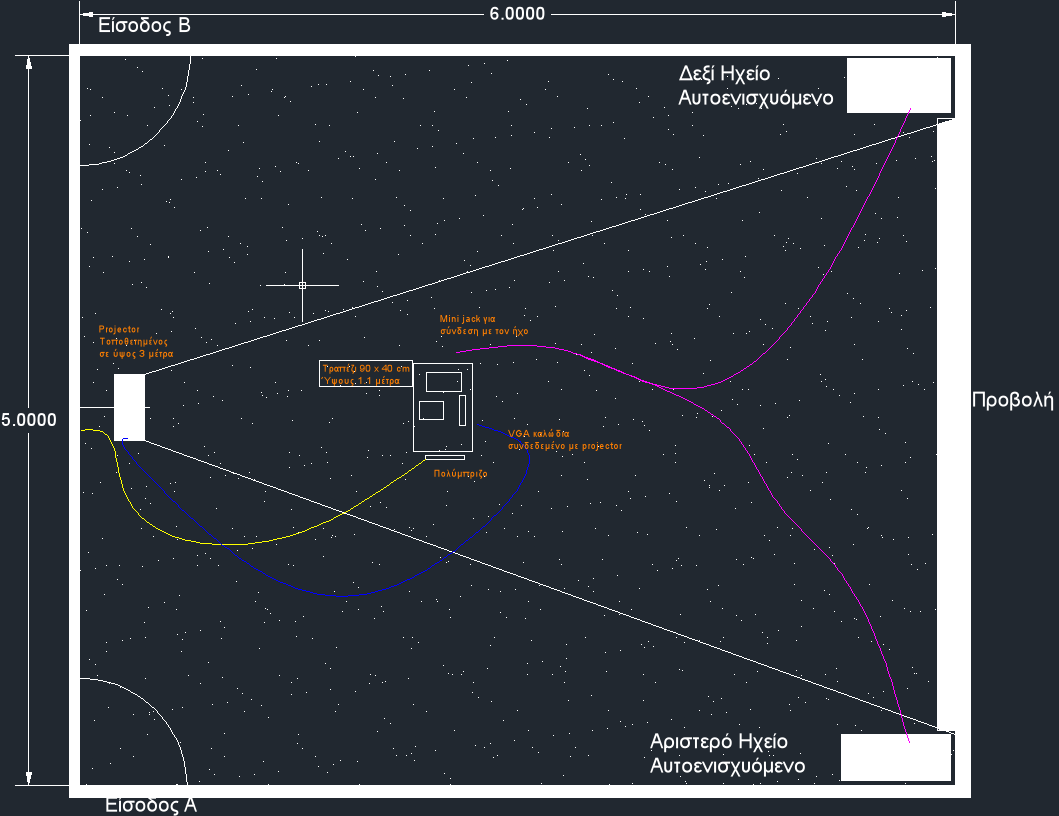
\includegraphics[width=10em]{./../installation/wireface_setup.png}
 
\section{Technics}
\label{sec-4}


\begin{itemize}
\item Όραση Υπολογιστών
\item Συναισθησία: διάδραση ήχου - εικόνας
\end{itemize}
\section{ScreenShots}
\label{sec-5}

\begin{center}

\end{center}
\section{About}
\label{sec-6}

\begin{itemize}
\item \href{http://wireface.com/}{WireFace official site}
\item \href{http://igoumeninja.org/}{igoumeninja} : Aris Bezas personal website
\item \href{http://earlab.org/}{EarLab} : Experimental Arts Laboratory (Iannis Zannos and \href{http://earlab.org/pmwiki.php?n=Members/HomePage}{members})
\item \href{http://iperatou.com/}{iperatou} : Interactive Audiovisual Performances by Dakis Trentos, Omer Chatziserif, Aris Bezas
\end{itemize}
\section{website}
\label{sec-7}

Ο ιστότοπος \href{http://wireface.com/}{http://wireface.com/} είναι σχεδιασμένος και προγραμματισμένος σε
\href{http://processingjs.org/}{ProcessingJS} η οποιά αποτελεί μια διεπαφή της \href{http://processing.org/}{Processing} για \href{http://en.wikipedia.org/wiki/JavaScript}{JavaScript}. 

\begin{itemize}
\item links:
\item \href{http://processingjs.org/reference/articles/RenderingModes}{Rendering Modes}
\end{itemize}
\section{Special thanks}
\label{sec-8}

\begin{itemize}
\item \href{https://github.com/ofTheo/ofxKinect}{Theodore Watson}
\item \href{http://forum.openframeworks.cc/index.php?topic=4947.0}{oF community}
\item \href{http://www.openframeworks.cc/}{openFrameworks}
\item \href{http://supercolliderbook.net/}{SuperCollider}
\item \href{http://earlab.org/}{Iannis Zannos}
\item \href{http://www.earslap.com/}{Batuhan Bozkurt}
\item \href{http://zepadovani.info}{José Henrique Padovani}
\end{itemize}

\end{document}
